\newpage


%%%%%%%%%%%%%%%%%%%%%%%%%%%%%%%%%%%%%%%%%%%%%%%%%%%%%%%%%%%%%%%%%%%%%%%%%%%%%%%%%%%%%%%
%%%%%%%%%%%%%%%%%%%%%%%%%%%%%%%%%%%%%%%%%%%%%%%%%%%%%%%%%%%%%%%%%%%%%%%%%%%%%%%%%%%%%%%
%%%%%%%%%%%%%%%%%%%%%%%%%%%%%%%%%%%%%%%%%%%%%%%%%%%%%%%%%%%%%%%%%%%%%%%%%%%%%%%%%%%%%%%
\section{\textcolor{red}{Regressão logística-fourier e SE com classificador $f_{\VECTOR{c}}(\VECTOR{x}):~\mathbb{R}^{N} \rightarrow \mathbb{R}$}}
\label{sec:theo:reglogrnr1fourier:1}

\index{Regressão!Logística $f_{\VECTOR{c}}(\VECTOR{x}):~\mathbb{R}^{N} \rightarrow \mathbb{R}$}

\begin{theorem}[Classificação de dados em $\mathbb{R}$:]\label{theo:reglogrnr1fourier:1}
~\\
\noindent
\begin{minipage}{0.45\textwidth}
\centering
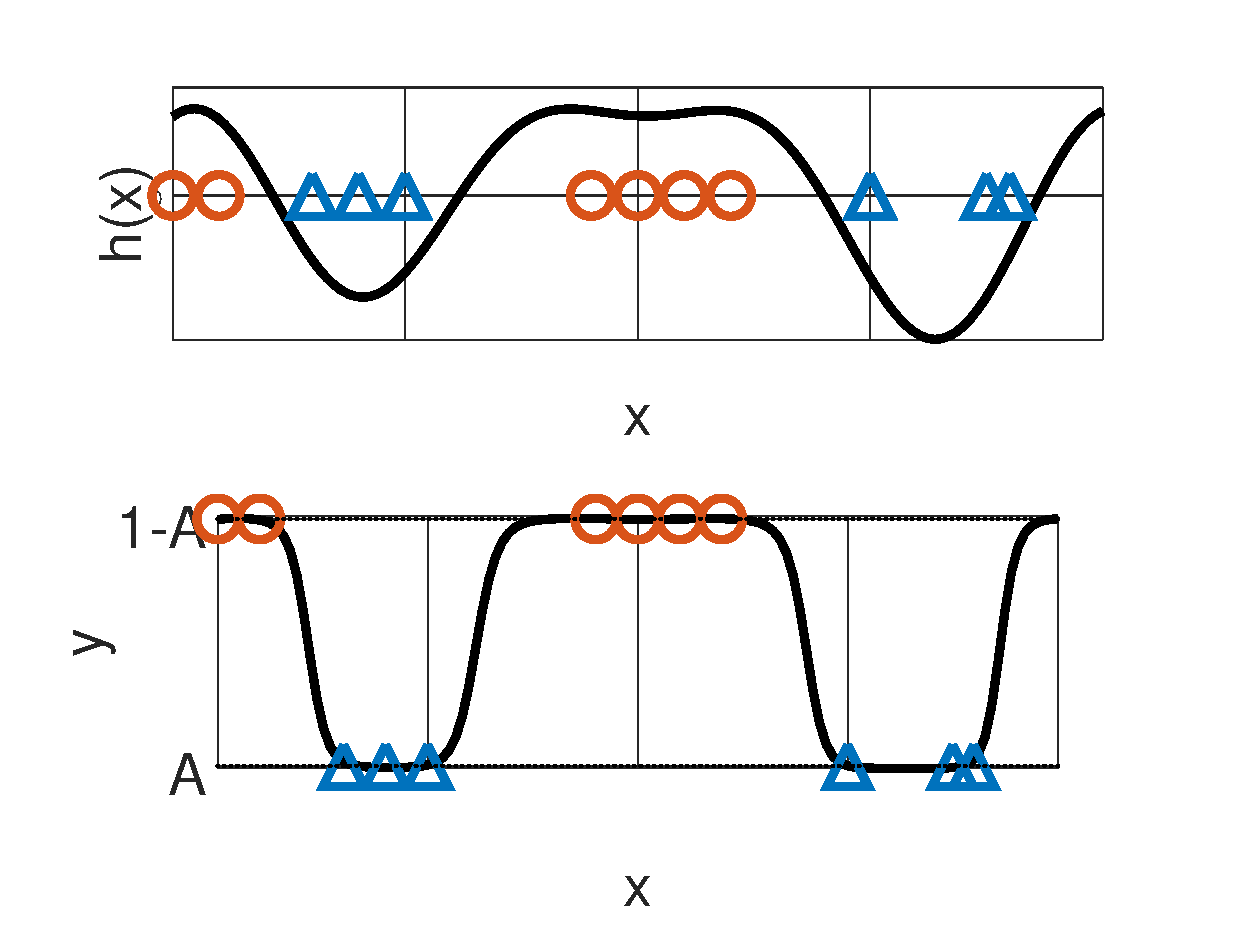
\includegraphics[width=0.95\linewidth]{chapters/classificacao/mfiles/reglogrnr1fourier/reglogrnr1fourier.eps} 
\end{minipage}
\begin{minipage}{0.55\textwidth}
Dados, um conjunto de $L$ pontos $\VECTOR{x}_l \in \mathbb{R}^{N} , 1 \leq l \leq L$,
repartidos em dois grupos etiquetados com os símbolos $\bigtriangleup$ e $\bigcirc$, 
não separáveis por um hiperplano.
Se desejamos criar um classificador mediante 
a função  $f_{\VECTOR{c}}:\mathbb{R}^{N} \rightarrow \mathbb{R}$,
com domínio $\VECTOR{x} \in \mathbb{R}^{N}$, contradomínio $y \in \mathbb{R}$ e 
parâmetros agrupados no vetor $\VECTOR{c}\in \mathbb{R}^{2 M+1}$, 
$M=\frac{(2 K+1)^N-1}{2}$,
como definido na Eq. (\ref{eq:reglogrnr1fourier:1}),
\begin{equation}\label{eq:reglogrnr1fourier:1}
y\equiv f_{\VECTOR{c}}(\VECTOR{x})= \frac{1}{1+e^{-h_{\VECTOR{c}}(\VECTOR{x}) }},
\end{equation}
\end{minipage}
\begin{equation}
 h_{\VECTOR{c}}(\VECTOR{x}) = a_{\VECTOR{k}_{0}}+
\sum_{m=1}^{M}
a_{\VECTOR{k}_{m}} cos\left(\VECTOR{x}^{\transpose}\MATRIX{W}_{L}\VECTOR{k}_{m}\right)+
b_{\VECTOR{k}_{m}} sin\left(\VECTOR{x}^{\transpose}\MATRIX{W}_{L}\VECTOR{k}_{m}\right),
\end{equation}
\begin{equation}
\VECTOR{c}=[
a_{\VECTOR{k}_{0}}\quad 
a_{\VECTOR{k}_{1}}\quad  
a_{\VECTOR{k}_{2}}\quad  
...\quad 
a_{\VECTOR{k}_{M}}\quad  
b_{\VECTOR{k}_{1}}\quad 
b_{\VECTOR{k}_{2}}\quad 
...\quad 
b_{\VECTOR{k}_{M}}
]^{\transpose},
\end{equation}
ou seu equivalente: $logit(y)=h_{\VECTOR{c}}(\VECTOR{x})$, onde a matriz
$\MATRIX{W}_{L}=\funcdiag\left(\left[\frac{2 \pi}{L_1},~\frac{2 \pi}{L_2},~\dots,~\frac{2 \pi}{L_N}\right]^{\transpose}\right)$
e\footnote{Tem 
que ser maior para evitar erros de $f_{\VECTOR{c}}(\VECTOR{x})$ nos extremos. 
Ex.: $L_n =1.1 || max(x_n)-min(x_n)||$.}
 $L_n > || max(x_n)-min(x_n)||$.

Podemos atribuir a cada vetor $\VECTOR{x}_l$ uma etiqueta $y_l\in \{A,1-A\}$, 
onde $0<A\ll 0.5$ é escolhido por nós,
e afirmar que o vetor $\VECTOR{c}= \VECTOR{\hat{c}}$,
que minimiza o erro quadrático $e(\VECTOR{c})$,
\begin{equation}\label{eq:reglogrnr1fourier:1e}
e(\VECTOR{c}) =  \sum_{l=1}^{L} q_l||h_{\VECTOR{c}}(\VECTOR{x}_l) -logit(y_l)||^2,
\end{equation}
ponderado usando os pesos $q_l \in \mathbb{R}_+$ agrupados na matriz 
$\MATRIX{Q}=\funcdiag \left([q_1\quad q_2\quad  \hdots \quad q_L ]^{\transpose}\right)$, 
pode ser achado\footnote{A demostração pode ser vista na Prova \ref{proof:theo:reglogrnr1fourier}.}  
com
\begin{equation}\label{eq:reglogrnr1fourier:2}
\VECTOR{\hat{c}} =  \left[ \MATRIX{A}^{\transpose} \MATRIX{Q}\MATRIX{A}\right]^{-1} \MATRIX{A}^{\transpose} \MATRIX{Q}\VECTOR{z},
\quad
\MATRIX{A}=
\begin{bmatrix}
1 & \VECTOR{\phi}_{K}(\VECTOR{x}_1) \\
1 & \VECTOR{\phi}_{K}(\VECTOR{x}_2) \\
%\vdots & \vdots \\
%1 & \VECTOR{\phi}_{K}(\VECTOR{x}_l) \\
\vdots & \vdots \\
1 & \VECTOR{\phi}_{K}(\VECTOR{x}_L) \\
\end{bmatrix},,
\quad
\VECTOR{z}=
\begin{bmatrix}
logit(y_1)  \\
logit(y_2)  \\
%\vdots  \\
%logit(y_l)  \\
\vdots \\
logit(y_L) \\
\end{bmatrix},
\end{equation}
\begin{equation}
\VECTOR{\phi}_{K}(\VECTOR{x})=
\begin{bmatrix}
cos\left(\VECTOR{x}^{\transpose}\MATRIX{W}_{L}\VECTOR{k}_{1}\right) &
\dots  &
cos\left(\VECTOR{x}^{\transpose}\MATRIX{W}_{L}\VECTOR{k}_{M}\right) &
%cos\left(\VECTOR{x}^{\transpose}\MATRIX{W}_{L}\VECTOR{k}_{2}\right) &
%sin\left(\VECTOR{x}^{\transpose}\MATRIX{W}_{L}\VECTOR{k}_{2}\right) &
sin\left(\VECTOR{x}^{\transpose}\MATRIX{W}_{L}\VECTOR{k}_{1}\right) &
\dots  &
sin\left(\VECTOR{x}^{\transpose}\MATRIX{W}_{L}\VECTOR{k}_{M}\right)
\end{bmatrix}.
\end{equation}
\end{theorem}
\begin{tcbattention}
\begin{itemize}
\item Dado que a função de classificação $f_{\VECTOR{c}}(\VECTOR{x})$ vai entre $0$ e $1$,
podemos reinterpretar este valor como se fosse uma probabilidade;
neste caso, $f_{\VECTOR{c}}(\VECTOR{x}_l)$ representa, $P(y_l=\bigcirc|\VECTOR{x}_l)$, 
a probabilidade de que $y_l=\bigcirc$ dado que tivemos como entrada o ponto $\VECTOR{x}_l$.
\end{itemize}
\end{tcbattention}
\begin{tcbattention}
\begin{itemize}
\item O limiar de classificação na função $f_{\VECTOR{c}}(\VECTOR{x})$ está na superfície $h_{\VECTOR{c}}(\VECTOR{x})=0$.
%provocando nestos pontos um $f_{\VECTOR{c}}(\VECTOR{x})=0.5$.
\item A ordem dos elementos do vetor $\VECTOR{\phi}_{k}(\VECTOR{x})$ podem ser alterados,
isto só modificará a posição dos elementos no vetor $\VECTOR{c}$.
\end{itemize}
\end{tcbattention}

\section{Provas}


\begin{myproofT}[Relativa ao Teorema \ref{sec:theo:reglogrnr1fourier:1}:]
\label{proof:theo:reglogrnr1fourier}
\textcolor{red}{Fingerprint a detectar surcos}\\
Se a função $h(\VECTOR{x}):~\mathbb{R}^{N} \rightarrow \mathbb{R}$,
\begin{equation}
h(\VECTOR{x}) = h(\VECTOR{x}+\VECTOR{r}),\qquad 
\VECTOR{r}=\left[L_1,~L_2,~\dots,~L_N\right]^{\transpose}
\end{equation}
é aproximada com uma 
version truncada da serie de fourier multivariable, 
onde o vetor de indices 
$\VECTOR{k}=[k_1\quad k_2\quad  ...\quad k_N]^{\transpose}$ tem valores entre 
$[-K\quad ...\quad-K]^{\transpose} \leq  \VECTOR{k}\leq [K\quad ...\quad K]^{\transpose}$,
como no exemplo da Tabela \ref{tab:theo:reglogrnr1fourier:2}; 
então podemos definir a seguinte equação
\begin{equation}\label{eq:proof:theo:reglogrnr1fourier:1}
 h(\VECTOR{x}) \approx
\sum_{\VECTOR{k}=[-K\quad ...\quad-K]^{\transpose}}^{[K\quad ...\quad K]^{\transpose}}
d_{\VECTOR{k}}  e^{\mathbf{i}\VECTOR{k}^{\transpose}\MATRIX{W}_{L}\VECTOR{x}}, 
\end{equation}
onde 
$\MATRIX{W}_{L}=\funcdiag\left(\left[\frac{2 \pi}{L_1},~\frac{2 \pi}{L_2},~\dots,~\frac{2 \pi}{L_N.}\right]^{\transpose}\right)$.
Se reordenamos a Eq. (\ref{eq:proof:theo:reglogrnr1fourier:1}) obtemos
\begin{equation}
 h(\VECTOR{x}) \approx d_{\VECTOR{0}}+
\sum_{\VECTOR{k}=[1,~0, ...,0]}^{[K,~K,~ ...,~K]}
d_{\VECTOR{k}}  e^{\mathbf{i}\VECTOR{k}^{\transpose}\MATRIX{W}_{L}\VECTOR{x}}
+
\sum_{\VECTOR{k}=[-K,~-K,~ ...,-K]}^{[-1,~0,~...,~0]}
d_{\VECTOR{k}}  e^{\mathbf{i}\VECTOR{k}^{\transpose}\MATRIX{W}_{L}\VECTOR{x}}.
\end{equation}
Para compactar a notação definimos $[1,~ 0,~ ...,~ 0 ]\equiv \mathbf{\bar{1}}$
e $[K,~ K,~ ...,~K ]\equiv \mathbf{\bar{K}}$,
\begin{equation}
 h(\VECTOR{x}) \approx d_{\VECTOR{0}}+
\sum_{\VECTOR{k}=\mathbf{\bar{1}}}^{\mathbf{\bar{K}}}
d_{\VECTOR{k}}  e^{\mathbf{i}\VECTOR{k}^{\transpose}\MATRIX{W}_{L}\VECTOR{x}}
+
\sum_{\VECTOR{k}=-\mathbf{\bar{1}}}^{-\mathbf{\bar{K}}}
d_{\VECTOR{k}}  e^{\mathbf{i}\VECTOR{k}^{\transpose}\MATRIX{W}_{L}\VECTOR{x}},
\end{equation}

\begin{equation}
 h(\VECTOR{x}) \approx d_{\VECTOR{0}}+
\sum_{\VECTOR{k}=\mathbf{\bar{1}}}^{\mathbf{\bar{K}}}
d_{\VECTOR{k}}  e^{\mathbf{i}\VECTOR{k}^{\transpose}\MATRIX{W}_{L}\VECTOR{x}}
+
\sum_{\VECTOR{k}=\mathbf{\bar{1}}}^{\mathbf{\bar{K}}}
d_{-\VECTOR{k}}  e^{-\mathbf{i}\VECTOR{k}^{\transpose}\MATRIX{W}_{L}\VECTOR{x}},
\end{equation}

\begin{equation}
 h(\VECTOR{x}) \approx d_{\VECTOR{0}}+
\sum_{\VECTOR{k}=\mathbf{\bar{1}}}^{\mathbf{\bar{K}}}
\left(d_{\VECTOR{k}}+d_{-\VECTOR{k}}\right) ~ cos\left(\VECTOR{k}^{\transpose}\MATRIX{W}_{L}\VECTOR{x}\right)+
\left(d_{\VECTOR{k}}-d_{-\VECTOR{k}}\right)~ \mathbf{i}~ sin\left(\VECTOR{k}^{\transpose}\MATRIX{W}_{L}\VECTOR{x}\right),
\end{equation}

\begin{equation}
 h(\VECTOR{x}) \approx d_{\VECTOR{0}}+
\sum_{\VECTOR{k}=\mathbf{\bar{1}}}^{\mathbf{\bar{K}}}
 2~Re\left\{d_{\VECTOR{k}}\right\}~ cos\left(\VECTOR{k}^{\transpose}\MATRIX{W}_{L}\VECTOR{x}\right)
-2~Im\left\{d_{\VECTOR{k}}\right\}~ sin\left(\VECTOR{k}^{\transpose}\MATRIX{W}_{L}\VECTOR{x}\right).
\end{equation}

Se fazemos uma troca de variaveis 
$a_{\VECTOR{0}}=d_{\VECTOR{0}}$,  
$a_{\VECTOR{k}}=2~Re\left\{d_{\VECTOR{k}}\right\}$ e
$b_{\VECTOR{k}}=-2~Im\left\{d_{\VECTOR{k}}\right\}$ 
\begin{equation}
\label{eq:proof:theo:reglogrnr1fourier:10}
 h(\VECTOR{x}) \approx a_{\VECTOR{0}}+
\sum_{\VECTOR{k}=\mathbf{\bar{1}}}^{\mathbf{\bar{K}}}
a_{\VECTOR{k}}~ cos\left(\VECTOR{k}^{\transpose}\MATRIX{W}_{L}\VECTOR{x}\right)
+b_{\VECTOR{k}}~ sin\left(\VECTOR{k}^{\transpose}\MATRIX{W}_{L}\VECTOR{x}\right).
\end{equation}

Seguindo a Tabela \ref{tab:theo:reglogrnr1fourier:1}, podemos observar que o 
número $M$ de vetores $\VECTOR{k}$ desde $\VECTOR{k}_{1}\equiv\mathbf{\bar{1}}\in \mathbb{R}^N$ ate 
$\VECTOR{k}_{M}\equiv\mathbf{\bar{K}}\in \mathbb{R}^N$ é igual a
\begin{equation}
M=\frac{(2K+1)^N-1}{2},
\end{equation}
de modo que podemos recrever a Eq. (\ref{eq:proof:theo:reglogrnr1fourier:10}) como
\begin{equation}
 h(\VECTOR{x}) \approx a_{\VECTOR{k}_{0}}+
\sum_{m=1}^{M}
 a_{\VECTOR{k}_{m}}~ cos\left(\VECTOR{x}^{\transpose}\MATRIX{W}_{L}\VECTOR{k}_{m}\right)
+b_{\VECTOR{k}_{m}}~ sin\left(\VECTOR{x}^{\transpose}\MATRIX{W}_{L}\VECTOR{k}_{m}\right).
\end{equation}
\end{myproofT}

\noindent
\begin{minipage}{0.45\textwidth}
\begin{table}[H]
\centering
\begin{tabular}{|l||r|r|}
\hline
$\VECTOR{k}_m$     &$k_1^{(m)}$& $k_2^{(m)}$      \\ \hline \hline
$\VECTOR{k}_{-12}$ & -2 & -2 \\ \hline
$\VECTOR{k}_{-11}$ & -1 & -2 \\ \hline
$\VECTOR{k}_{-10}$ &  0 & -2 \\ \hline
$\VECTOR{k}_{-9}$  &  1 & -2 \\ \hline
$\VECTOR{k}_{-8}$  &  2 & -2 \\ \hline \hline
$\VECTOR{k}_{-7}$  & -2 & -1 \\ \hline 
$\VECTOR{k}_{-6}$  & -1 & -1 \\ \hline
$\VECTOR{k}_{-5}$  &  0 & -1 \\ \hline
$\VECTOR{k}_{-4}$  &  1 & -1 \\ \hline
$\VECTOR{k}_{-3}$  &  2 & -1 \\ \hline \hline
$\VECTOR{k}_{-2}$  & -2 &  0 \\ \hline
$\VECTOR{k}_{-1}$  & -1 &  0 \\ \hline
$\VECTOR{k}_{0}$   & $\mathbf{0}$ & $\mathbf{0}$ \\ \hline
$\VECTOR{k}_{1}$   &  1 &  0 \\ \hline
$\VECTOR{k}_{2}$   &  2 &  0 \\ \hline \hline
$\VECTOR{k}_{3}$   & -2 &  1 \\ \hline
$\VECTOR{k}_{4}$   & -1 &  1 \\ \hline
$\VECTOR{k}_{5}$   &  0 &  1 \\ \hline
$\VECTOR{k}_{6}$   &  1 &  1 \\ \hline
$\VECTOR{k}_{7}$   &  2 &  1 \\ \hline \hline
$\VECTOR{k}_{8}$   & -2 &  2 \\ \hline
$\VECTOR{k}_{9}$   & -1 &  2 \\ \hline
$\VECTOR{k}_{10}$  &  0 &  2 \\ \hline
$\VECTOR{k}_{11}$  &  1 &  2 \\ \hline
$\VECTOR{k}_{12}$  &  2 &  2 \\ \hline
\end{tabular}
\caption{Contagem desde $\VECTOR{k}_{-M}$ 
ate $\VECTOR{k}_{M}$ com $K=2$ e $N=2$.}
\label{tab:theo:reglogrnr1fourier:2}
\end{table}
\end{minipage}
\hfill
\begin{minipage}{0.45\textwidth}
\begin{table}[H]
\centering
\begin{tabular}{|l||l|l|l|l|}
\hline
$\VECTOR{k}_m$     &$k_1^{(m)}$& $k_2^{(m)}$      & $k_3^{(m)}$         & ...                   \\ \hline \hline
$\VECTOR{k}_{1}$   & 1      & \multirow{3}{*}{0}  & \multirow{11}{*}{0} & \multirow{20}{*}{...} \\ \cline{1-2}
\vdots             & \vdots &                     &                     &                       \\ \cline{1-2}
$\VECTOR{k}_{K}$   & K      &                     &                     &                       \\ \cline{1-3}
$\VECTOR{k}_{K+1}$ & -K     & \multirow{3}{*}{1}  &                     &                       \\ \cline{1-2}
\vdots             & \vdots &                     &                     &                       \\ \cline{1-2}
$\VECTOR{k}_{3K+1}$& K      &                     &                     &                       \\ \cline{1-3}
$\VECTOR{k}_{3K+2}$& -K     & \multirow{3}{*}{2}  &                     &                       \\ \cline{1-2}
\vdots             & \vdots &                     &                     &                       \\ \cline{1-2}
$\VECTOR{k}_{5K+2}$& K      &                     &                     &                       \\ \cline{1-3}
\vdots             & \vdots & \vdots              &                     &                       \\ \cline{1-3}
$\VECTOR{k}_{2K^2+2K}$  & K & K                   &                     &                       \\ \cline{1-4}
$\VECTOR{k}_{2K^2+2K+1}$& -K& \multirow{3}{*}{-K} & \multirow{7}{*}{1}  &                       \\ \cline{1-2}
\vdots             & \vdots &                     &                     &                       \\ \cline{1-2}
$\VECTOR{k}_{2K^2+4K+1}$& K &                     &                     &                       \\ \cline{1-3}
\vdots             & \vdots & \vdots              &                     &                       \\ \cline{1-3}
$\VECTOR{k}_{6K^2+4K+1}$& -K& \multirow{3}{*}{K}  &                     &                       \\ \cline{1-2}
\vdots             & \vdots &                     &                     &                       \\ \cline{1-2}
$\VECTOR{k}_{6K^2+6K+1}$& K &                     &                     &                       \\ \cline{1-4}
\vdots             & \vdots & \vdots              & \vdots              &                       \\ \cline{1-4}
$\VECTOR{k}_{M}$   & K      & K                   & K                   &                       \\ \hline
\end{tabular}
\caption{Contagem desde $\VECTOR{k}_{1}=[1,~ 0,~ ...,~ 0 ]\equiv \mathbf{\bar{1}}$ 
ate $\VECTOR{k}_{M}=[K,~ K,~ ...,~ K ]\equiv \mathbf{\bar{K}}$ com elementos $-K\leq k_n^{(m)}\leq K$.}
\label{tab:theo:reglogrnr1fourier:1}
\end{table}
\end{minipage}


